\subsection{Задача 2}
\subsubsection{а)}
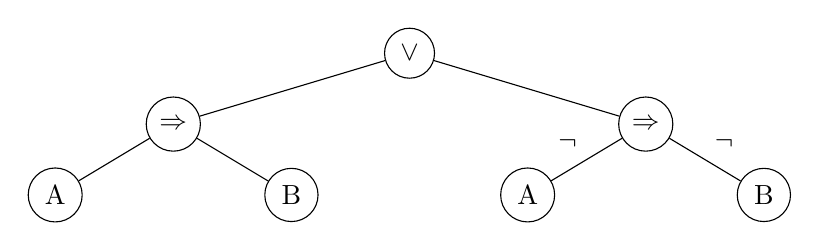
\begin{tikzpicture}[level/.style={sibling distance=100mm/#1}, scale=0.6]
\node [circle, draw=black] {$ \lor  $}
  child { 
    node [circle, draw=black] {$ \Rightarrow $}
    child {
      node [circle, draw=black] {A}
    }
    child {
      node [circle, draw=black] {B}
    }
  }
  child {
    node [circle, draw=black] {$ \Rightarrow  $} 
    child {
      node [circle, draw=black] {A}
      edge from parent node[above left] {$ \lnot  $}
    }
    child {
      node [circle, draw=black] {B}
      edge from parent node[above right] {$ \lnot  $}
    }
  };
\end{tikzpicture}

\rule{0cm}{0cm}

\begin{tabular}{|c|c|c|}
  \hline
  A & B & $ (A \Rightarrow B) \lor (\lnot A \Rightarrow \lnot B) $ \\ \hline
  0 & 0 & 1                                                        \\ \hline
  0 & 1 & 1                                                        \\ \hline
  1 & 0 & 1                                                        \\ \hline
  1 & 1 & 1                                                        \\ \hline
\end{tabular}


\subsubsection{б)}
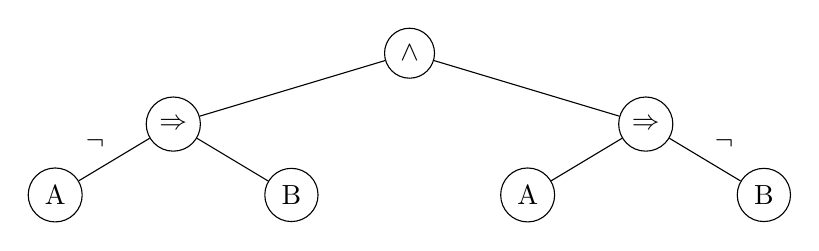
\begin{tikzpicture}[level/.style={sibling distance=100mm/#1}, scale=0.6]
\node [circle, draw=black] {$ \land  $}
  child {
    node [circle, draw=black] {$ \Rightarrow  $}
    child {
      node [circle, draw=black] {A}
      edge from parent node[above left] {$ \lnot  $}
    }
    child {
      node [circle, draw=black] {B}
    }
  }
  child {
    node [circle, draw=black] {$ \Rightarrow  $}
    child {
      node [circle, draw=black] {A}
    }
    child {
      node [circle, draw=black] {B}
      edge from parent node[above right] {$ \lnot  $}
    }
  };
\end{tikzpicture}

\rule{0cm}{0cm}

\begin{tabular}{|c|c|c|}
  \hline
  A & B & $ (\lnot A \Rightarrow B) \land (A \Rightarrow \lnot B) $ \\ \hline
  0 & 0 & 0                                                         \\ \hline
  0 & 1 & 1                                                         \\ \hline
  1 & 0 & 1                                                         \\ \hline
  1 & 1 & 0                                                         \\ \hline
\end{tabular}


\subsubsection{в)}
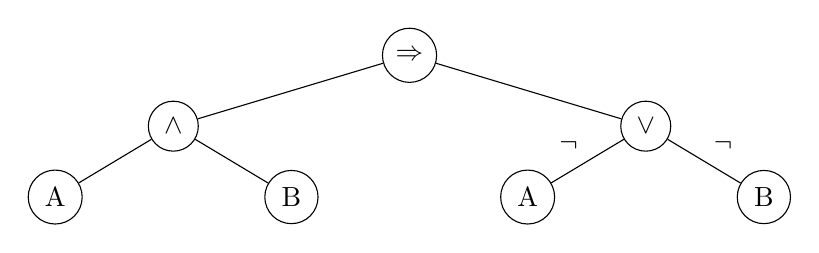
\begin{tikzpicture}[level/.style={sibling distance=100mm/#1}, scale=0.6]
\node [circle, draw=black] {$ \Rightarrow  $}
  child { 
    node [circle, draw=black] {$ \land  $}
    child {
      node [circle, draw=black] {A}
    }
    child {
      node [circle, draw=black] {B}
    }
  }
  child {
    node [circle, draw=black] {$ \lor  $}
    child {
      node [circle, draw=black] {A}
      edge from parent node[above left] {$ \lnot  $}
    }
    child {
      node [circle, draw=black] {B}
      edge from parent node[above right] {$ \lnot  $}
    }
  };
\end{tikzpicture}

\rule{0cm}{0cm}

\begin{tabular}{|c|c|c|}
  \hline
  A & B & $ (A \land B) \Rightarrow (\lnot A \lor \lnot B) $ \\ \hline
  0 & 0 & 1                                                  \\ \hline
  0 & 1 & 1                                                  \\ \hline
  1 & 0 & 1                                                  \\ \hline
  1 & 1 & 0                                                  \\ \hline
\end{tabular}


\subsubsection{г)}
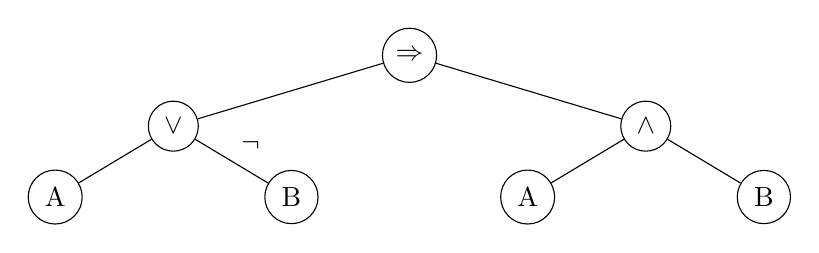
\begin{tikzpicture}[level/.style={sibling distance=100mm/#1}, scale=0.6]
\node [circle, draw=black] {$ \Rightarrow  $}
  child { 
    node [circle, draw=black] {$ \lor  $}
    child {
      node [circle, draw=black] {A}
    }
    child {
      node [circle, draw=black] {B}
      edge from parent node[above right]{$ \lnot  $}
    }
  }
  child {
    node [circle, draw=black] {$ \land  $}
    child {
      node [circle, draw=black] {A}
    }
    child {
      node [circle, draw=black] {B}
    }
  };
\end{tikzpicture}

\rule{0cm}{0cm}

\begin{tabular}{|c|c|c|}
  \hline
  A & B & $ (A \lor \lnot B) \Rightarrow (A \land B) $ \\ \hline
  0 & 0 & 0                                                  \\ \hline
  0 & 1 & 1                                                  \\ \hline
  1 & 0 & 0                                                  \\ \hline
  1 & 1 & 1                                                  \\ \hline
\end{tabular}


\subsubsection{д)}
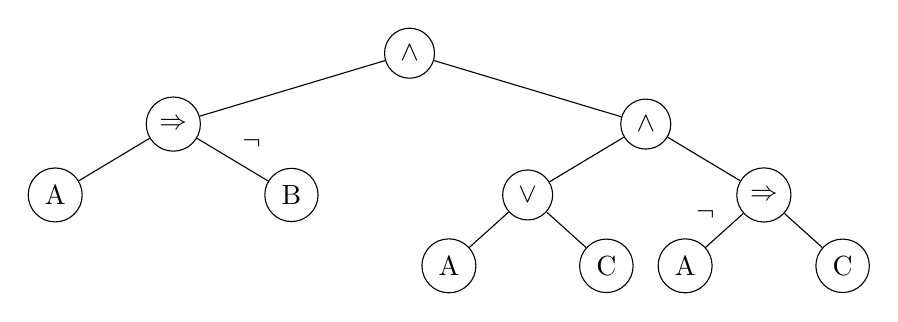
\begin{tikzpicture}[level/.style={sibling distance=100mm/#1}, scale=0.6]
\node [circle, draw=black] {$ \land  $}
  child { 
    node [circle, draw=black] {$ \Rightarrow  $}
    child {
      node [circle, draw=black] {A}
    }
    child {
      node [circle, draw=black] {B}
      edge from parent node[above right] {$ \lnot $}
    }
  }
  child {
    node [circle, draw=black] {$ \land  $}
    child {
      node [circle, draw=black] {$ \lor  $}
      child {
        node [circle, draw=black] {A}
      }
      child {
        node [circle, draw=black] {C}
      }
    }
    child {
      node [circle, draw=black] {$ \Rightarrow  $}
      child {
        node [circle, draw=black] {A}
        edge from parent node[above left] {$ \lnot  $}
      }
      child {
        node [circle, draw=black] {C}
      }
    }
  };
\end{tikzpicture}

\rule{0cm}{0cm}

\begin{tabular}{|c|c|c|c|}
  \hline
  A & B & C & $ (A \Rightarrow \lnot B) \land (A \lor C) \land (\lnot A \Rightarrow C) $ \\ \hline
  0 & 0 & 0 & 0                                                                          \\ \hline
  0 & 0 & 1 & 1                                                                          \\ \hline
  0 & 1 & 0 & 0                                                                          \\ \hline
  0 & 1 & 1 & 1                                                                          \\ \hline
  1 & 0 & 0 & 1                                                                          \\ \hline
  1 & 0 & 1 & 1                                                                          \\ \hline
  1 & 1 & 0 & 0                                                                          \\ \hline
  1 & 1 & 1 & 0                                                                          \\ \hline
\end{tabular}


\subsubsection{е)}
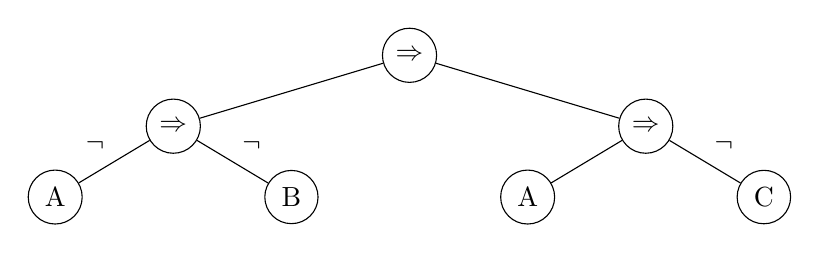
\begin{tikzpicture}[level/.style={sibling distance=100mm/#1}, scale=0.6]
\node [circle, draw=black] {$ \Rightarrow  $}
  child { 
    node [circle, draw=black] {$ \Rightarrow  $}
    child {
      node [circle, draw=black] {A}
      edge from parent node[above left] {$ \lnot  $}
    }
    child {
      node [circle, draw=black] {B}
      edge from parent node[above right] {$ \lnot  $}
    }
  }
  child { 
    node [circle, draw=black] {$ \Rightarrow  $}
    child {
      node [circle, draw=black] {A}
    }
    child {
      node [circle, draw=black] {C}
      edge from parent node[above right] {$ \lnot  $}
    }
  };
\end{tikzpicture}

\rule{0cm}{0cm}

\begin{tabular}{|c|c|c|c|}
  \hline
  A & B & C & $ (\lnot A \Rightarrow \lnot B) \Rightarrow (A \Rightarrow \lnot C) $ \\ \hline
  0 & 0 & 0 & 1                                                                     \\ \hline
  0 & 0 & 1 & 1                                                                     \\ \hline
  0 & 1 & 0 & 1                                                                     \\ \hline
  0 & 1 & 1 & 1                                                                     \\ \hline
  1 & 0 & 0 & 1                                                                     \\ \hline
  1 & 0 & 1 & 0                                                                     \\ \hline
  1 & 1 & 0 & 1                                                                     \\ \hline
  1 & 1 & 1 & 0                                                                     \\ \hline
\end{tabular}


\subsubsection{ж)}
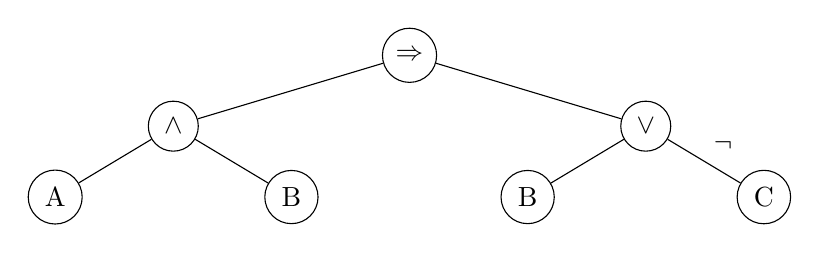
\begin{tikzpicture}[level/.style={sibling distance=100mm/#1}, scale=0.6]
\node [circle, draw=black] {$ \Rightarrow  $}
  child { 
    node [circle, draw=black] {$ \land  $}
    child {
      node [circle, draw=black] {A}
    }
    child {
      node [circle, draw=black] {B}
    }
  }
  child {
    node [circle, draw=black] {$ \lor  $}
    child {
      node [circle, draw=black] {B}
    }
    child {
      node [circle, draw=black] {C}
      edge from parent node[above right] {$ \lnot  $}
    }
  };
\end{tikzpicture}

\rule{0cm}{0cm}

\begin{tabular}{|c|c|c|c|}
  \hline
  A & B & C & $ A \land B \Rightarrow (B \lor \lnot C) $ \\ \hline
  0 & 0 & 0 & 1                                          \\ \hline
  0 & 0 & 1 & 1                                          \\ \hline
  0 & 1 & 0 & 1                                          \\ \hline
  0 & 1 & 1 & 1                                          \\ \hline
  1 & 0 & 0 & 1                                          \\ \hline
  1 & 0 & 1 & 0                                          \\ \hline
  1 & 1 & 0 & 1                                          \\ \hline
  1 & 1 & 1 & 0                                          \\ \hline
\end{tabular}


\subsubsection{з)}
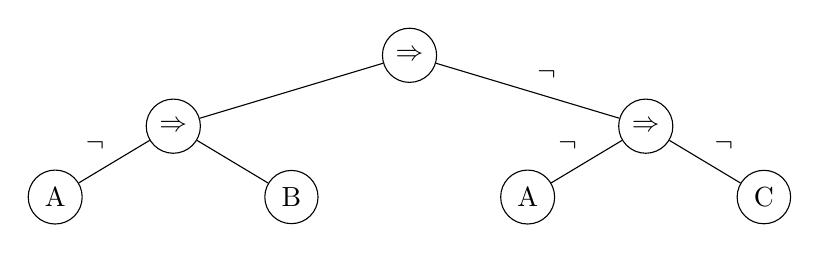
\begin{tikzpicture}[level/.style={sibling distance=100mm/#1}, scale=0.6]
\node [circle, draw=black] {$ \Rightarrow  $}
  child { 
    node [circle, draw=black] {$ \Rightarrow  $}
    child {
      node [circle, draw=black] {A}
      edge from parent node[above left] {$ \lnot  $}
    }
    child {
      node [circle, draw=black] {B}
    }
  }
  child {
    node [circle, draw=black] {$ \Rightarrow  $}
    child {
      node [circle, draw=black] {A}
      edge from parent node[above left] {$ \lnot  $}
    }
    child {
      node [circle, draw=black] {C}
      edge from parent node[above right] {$ \lnot  $}
    }
    edge from parent node[above right] {$ \lnot  $}
  };
\end{tikzpicture}

\rule{0cm}{0cm}

\begin{tabular}{|c|c|c|c|}
  \hline
  A & B & C & $ (\lnot A \Rightarrow B) \Rightarrow \lnot (\lnot A \Rightarrow \lnot C) $ \\ \hline
  0 & 0 & 0 & 1                                                                           \\ \hline
  0 & 0 & 1 & 1                                                                           \\ \hline
  0 & 1 & 0 & 0                                                                           \\ \hline
  0 & 1 & 1 & 1                                                                           \\ \hline
  1 & 0 & 0 & 0                                                                           \\ \hline
  1 & 0 & 1 & 0                                                                           \\ \hline
  1 & 1 & 0 & 0                                                                           \\ \hline
  1 & 1 & 1 & 0                                                                           \\ \hline
\end{tabular}


\subsubsection{и)}
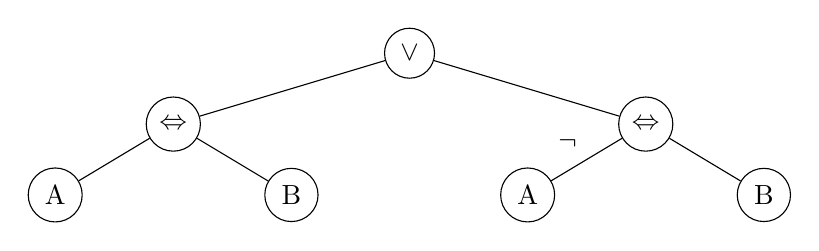
\begin{tikzpicture}[level/.style={sibling distance=100mm/#1}, scale=0.6]
\node [circle, draw=black] {$ \lor $}
  child { 
    node [circle, draw=black] {$ \Leftrightarrow $}
    child {
      node [circle, draw=black] {A}
    }
    child {
      node [circle, draw=black] {B}
    }
  }
  child {
    node [circle, draw=black] {$ \Leftrightarrow  $}
    child {
      node [circle, draw=black] {A}
      edge from parent node[above left] {$ \lnot  $}
    }
    child {
      node [circle, draw=black] {B}
    }
  };
\end{tikzpicture}

\rule{0cm}{0cm}

\begin{tabular}{|c|c|c|}
  \hline
  A & B & $ (A \Leftrightarrow B) \lor (\lnot A \Leftrightarrow B) $ \\ \hline
  0 & 0 & 1                                                          \\ \hline
  0 & 1 & 1                                                          \\ \hline
  1 & 0 & 1                                                          \\ \hline
  1 & 1 & 1                                                          \\ \hline
\end{tabular}


\subsubsection{к)}
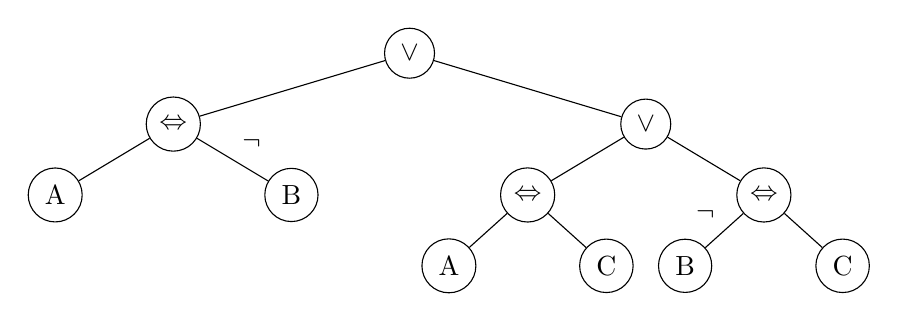
\begin{tikzpicture}[level/.style={sibling distance=100mm/#1}, scale=0.6]
\node [circle, draw=black] {$ \lor  $}
  child { 
    node [circle, draw=black] {$ \Leftrightarrow  $}
    child {
      node [circle, draw=black] {A}
    }
    child {
      node [circle, draw=black] {B}
      edge from parent node[above right] {$ \lnot  $}
    }
  }
  child {
    node [circle, draw=black] {$ \lor  $}
    child {
      node [circle, draw=black] {$ \Leftrightarrow  $}
      child {
        node [circle, draw=black] {A}
      }
      child {
        node [circle, draw=black] {C}
      }
    }
    child {
      node [circle, draw=black] {$ \Leftrightarrow  $}
      child {
        node [circle, draw=black] {B}
        edge from parent node[above left] {$ \lnot  $}
      }
      child {
        node [circle, draw=black] {C}
      }
    }
  };
\end{tikzpicture}

\rule{0cm}{0cm}

\begin{tabular}{|c|c|c|c|}
  \hline
  A & B & C & $ (A \Leftrightarrow B) \lor (A \Leftrightarrow C) \lor (\lnot B \Leftrightarrow C) $ \\ \hline
  0 & 0 & 0 & 1                                                                                     \\ \hline
  0 & 0 & 1 & 1                                                                                     \\ \hline
  0 & 1 & 0 & 1                                                                                     \\ \hline
  0 & 1 & 1 & 1                                                                                     \\ \hline
  1 & 0 & 0 & 1                                                                                     \\ \hline
  1 & 0 & 1 & 1                                                                                     \\ \hline
  1 & 1 & 0 & 1                                                                                     \\ \hline
  1 & 1 & 1 & 1                                                                                     \\ \hline
\end{tabular}
